% Intended LaTeX compiler: xelatex
\documentclass[11pt]{article}
\usepackage{graphicx}
\usepackage{longtable}
\usepackage{wrapfig}
\usepackage{rotating}
\usepackage[normalem]{ulem}
\usepackage{amsmath}
\usepackage{amssymb}
\usepackage{capt-of}
\usepackage{hyperref}
\author{Jacob Debel}
\date{Fysik B}
\title{Elektricitet}
\hypersetup{
 pdfauthor={Jacob Debel},
 pdftitle={Elektricitet},
 pdfkeywords={},
 pdfsubject={},
 pdfcreator={Emacs 29.4 (Org mode 9.6.15)}, 
 pdflang={Danish}}
\begin{document}

\maketitle

\section*{Elektrisk ladning}
\label{sec:org054cb49}
\subsection*{Av for Søren}
\label{sec:org5be59ea}
\begin{itemize}
\item Eksperimenter lidt. Hvad kan I finde ud af?
\end{itemize}

\subsection*{Dette kender I også}
\label{sec:org1b43472}
\begin{itemize}
\item Hvad skal I gøre, for at kunne skubbe til den ene ballon med den anden ballon?
\end{itemize}

\subsection*{Ladninger}
\label{sec:org7990c51}
\begin{itemize}
\item Symbolet for ladning er \(Q\) og måles i SI-enheden \(C\) (Coulomb).
\item En \textbf{elementarladning} er \(e=1.6 \cdot 10^{-19} \,C\).
\item En \textbf{elektron} har en ladning på \(-e\), mens en \textbf{proton} har en ladning på \(+e\).
\item Ladninger med \textbf{samme} fortegn \textbf{frastøder} hinanden.
\item Ladninger med \textbf{forskellige} fortegn \textbf{tiltrækker} hinanden.
\end{itemize}
\textbf{Opgave 13.1}

En kobberkugle har en nettoladning på 50 nC.

\begin{itemize}
\item Beregn, hvor mange elektroner det svarer til.
\end{itemize}

\textbf{Opgave 13.2}

\begin{itemize}
\item Hvor stor en nettoladning har ét mol enkeltladede ioner?
\end{itemize}

\subsection*{Coulombs lov}
\label{sec:org5daf78e}
I skal undersøge, hvordan den elektriske kraft mellem to ladninger afhænger af ladningernes størrelse (og fortegn) samt afstanden mellem ladningerne.

I må kun variere på en størrelse ad gangen. I kan derfor f.eks. gøre følgende:

\begin{enumerate}
\item Vælg atomic scale.
\item Flyt \(q_1\) ud til 0 pm og \(q_2\) til f.eks. 10 pm. Vælg \(q_1=1e\) og \(q_2=1e\).
\item Forøg nu gradvist ladningen på \(q_2\) og noter sammenhørende værdier af kraften.
\item Vælg nu to faste ladninger til \(q_1\) og \(q_2\), men varier afstanden mellem ladningerner. Noter sammenhørende værdier mellem afstand og kraft.
\item Plot jeres data i en række x,y-kooridatsystemer og undersøg vha regression, hvilke funktionstyper, som passer bedst til graferne.
\end{enumerate}

\subsection*{Coulombs lov}
\label{sec:org5e74341}
$$F = k \cdot \frac{Q_1\cdot Q_2}{r^2}\,,$$

hvor \(k=8.988 \cdot 10^9 \frac{N \cdot m^2}{C^2}\) kaldes \emph{Coulombs konstant}, \(Q_1\) og \(Q_2\) er ladningernes størrelse og \(r\) er afstanden mellem ladningerne. Hvis fortegnet på den elektriske kraft er positiv er, frastøder de to ladninger hinanden, og hvis fortegnet er negativt, tiltrækker de hinanden.

\subsection*{Elektriske felter}
\label{sec:orgcb6dd17}
Det elektriske \emph{felt} omkring en ladning \(Q\) er givet ved

$$E = k \cdot \frac{Q}{r^2}\,.$$

Feltstyrken måles i enheden \(\frac{V}{m}\) (volt pr. meter).

Den elektriske kraft på en \emph{testladning} \(q\) er da

$$F = q \cdot E\,.$$

\subsection*{Opgave 13.7}
\label{sec:org1d64e63}
\begin{enumerate}
\item Bestem den elektriske kraft mellem en heliumkerne og en elektron i afstanden \(1.3\cdot 10^{-10}m\)
\item Bestem feltstyrken fra heliumkernen i samme afstand.
\item Bestem gravitationskraften mellem heliumkernen og elektronen. Brug Newtons universelle gravitationslov
$$F_G = G \cdot \frac{M \cdot m}{r^2}\,,$$
Hvor \(G= 6.67\cdot 10^{-11} \frac{N \cdot m^2}{kg^2}\) er Newtons universelle gravitationskonstant, \(M\) og \(m\) er masserne af to objekter, mens \(r\) er afstanden mellem de to samme objekter.
\end{enumerate}

\section*{Strøm, spænding og energi}
\label{sec:org6ff277e}
\subsection*{Strøm(styrke)}
\label{sec:org7b635a5}
Ikke AI

men

$$\left[ I \right] = A$$

\subsubsection*{AC/DC \underline{Live} on stage!!}
\label{sec:org5174897}
\url{./img/ac\_dc.gif}

\href{https://youtu.be/v2AC41dglnM}{Musikvideo}

\subsubsection*{Opsummering}
\label{sec:org3980df7}
\begin{center}
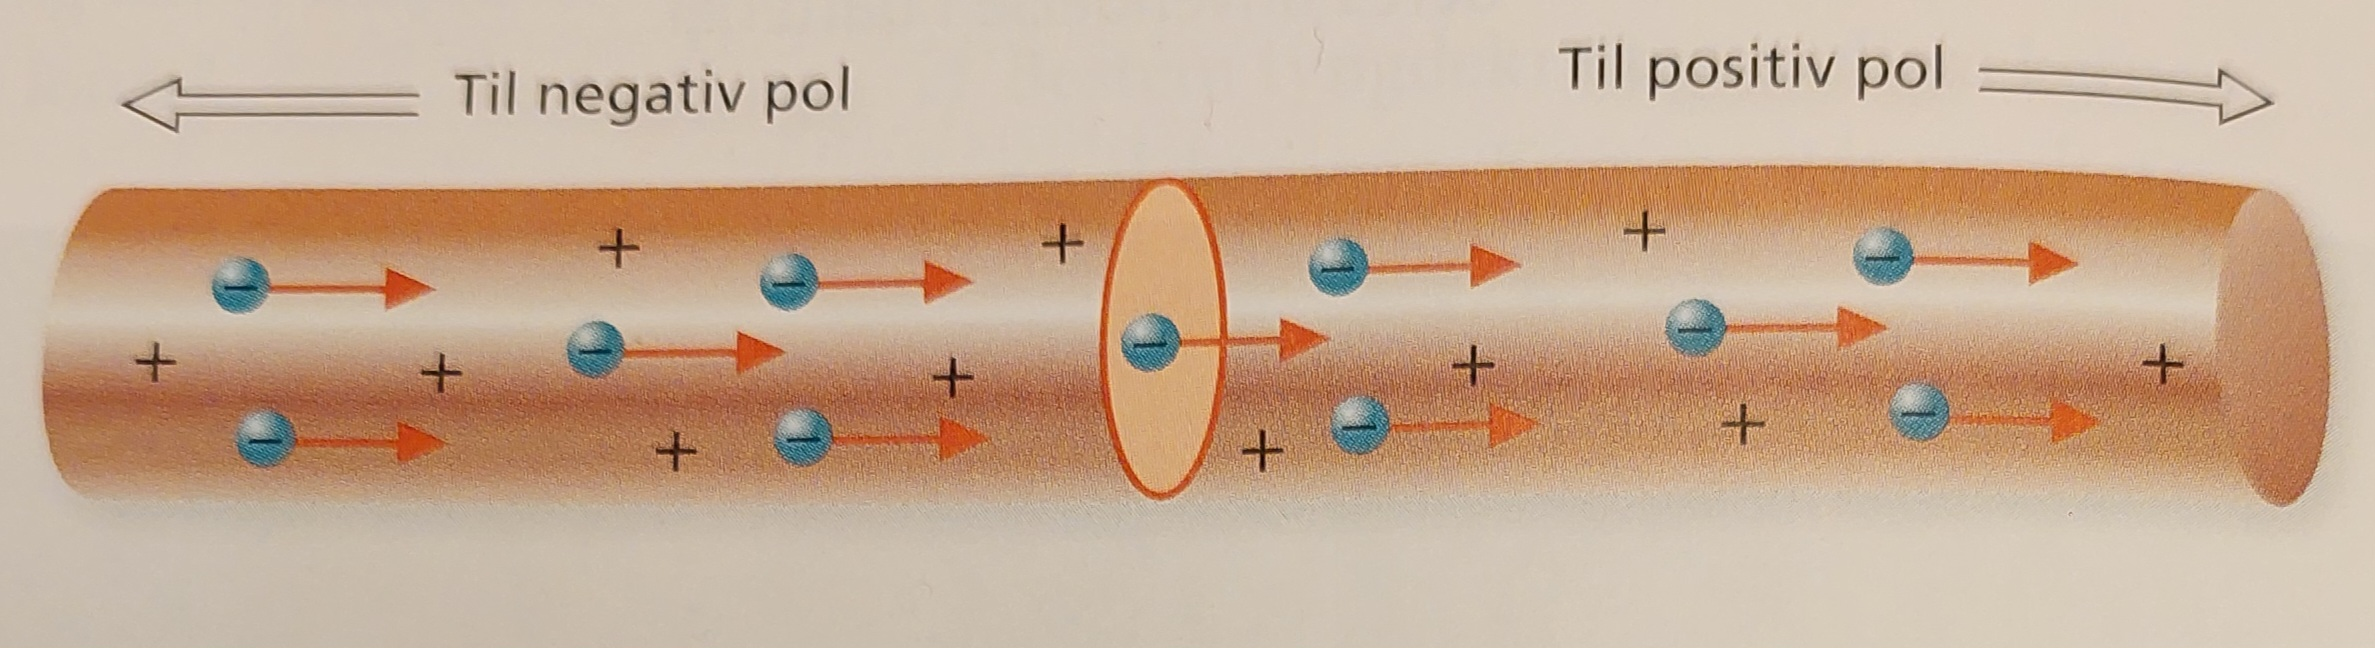
\includegraphics[width=.9\linewidth]{./img/stroem_01.jpg}
\end{center}
\begin{center}
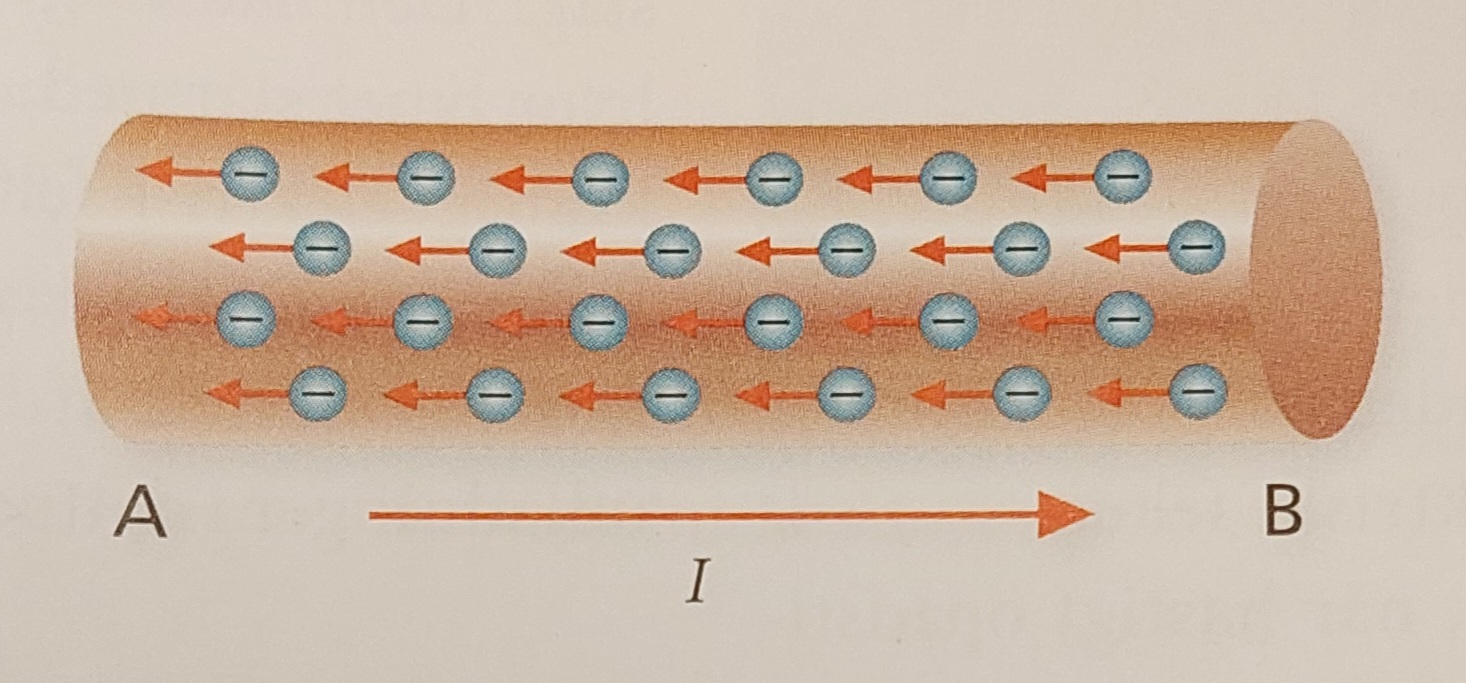
\includegraphics[width=.9\linewidth]{./img/stroem_02.jpg}
\end{center}
$$\boxed{I = \frac{\Delta Q}{\Delta t}}$$
\begin{itemize}
\item Antal ladninger som passerer et givent tværsnit i en leder(ledning) per tid.
\item Enheden for strøm(styrke) hedder \emph{ampere} og skrives som A.
\item Per definition løber strømmen fra den positive pol til den negative pol. I virkeligheden er det elektronerne, som vandrer fra den negative pol mod den positive pol.
\end{itemize}

\subsubsection*{Opgaver}
\label{sec:org740e03a}
\textbf{14.1}

I et lyn overføres ladningen 20 C mellem skyen og Jorden. \textbf{Hvor stor var den gennemsnitslige strømstyrke, hvis lynes varede 1.2 ms}?

\textbf{14.2}

Gennem et tværsnit af en leder passerer i løbet af 10 sekunder elektroner med en samlet ladning på -30 C. \textbf{Hvor stor er strømmen}?
\textbf{14.3}

Gennem en leder går en strøm på 8.0 A. \textbf{Hvor stor en ladning passere gennem et tværsnit af lederen i løbet af et minut}?


\textbf{14.4}

En tokamak er en maskine til at fastholde et plasma (ioner og elektroner). Inde i kammeret flyder ladede ioner rundt om centrum. Et tværsnit i maskinens kammer passeres hvert sekund af \(8.12 \cdot 10^{24}\) elektroner. \textbf{Hvor stor er strømstyrken i plasmaet}?

\subsection*{Spænding(sforskel)}
\label{sec:org88a259e}

\url{./img/scared.gif}

Arh ikke helt sådan noget spænding.

\subsection*{Spænding(sforskel)}
\label{sec:org080f1fc}
\begin{center}
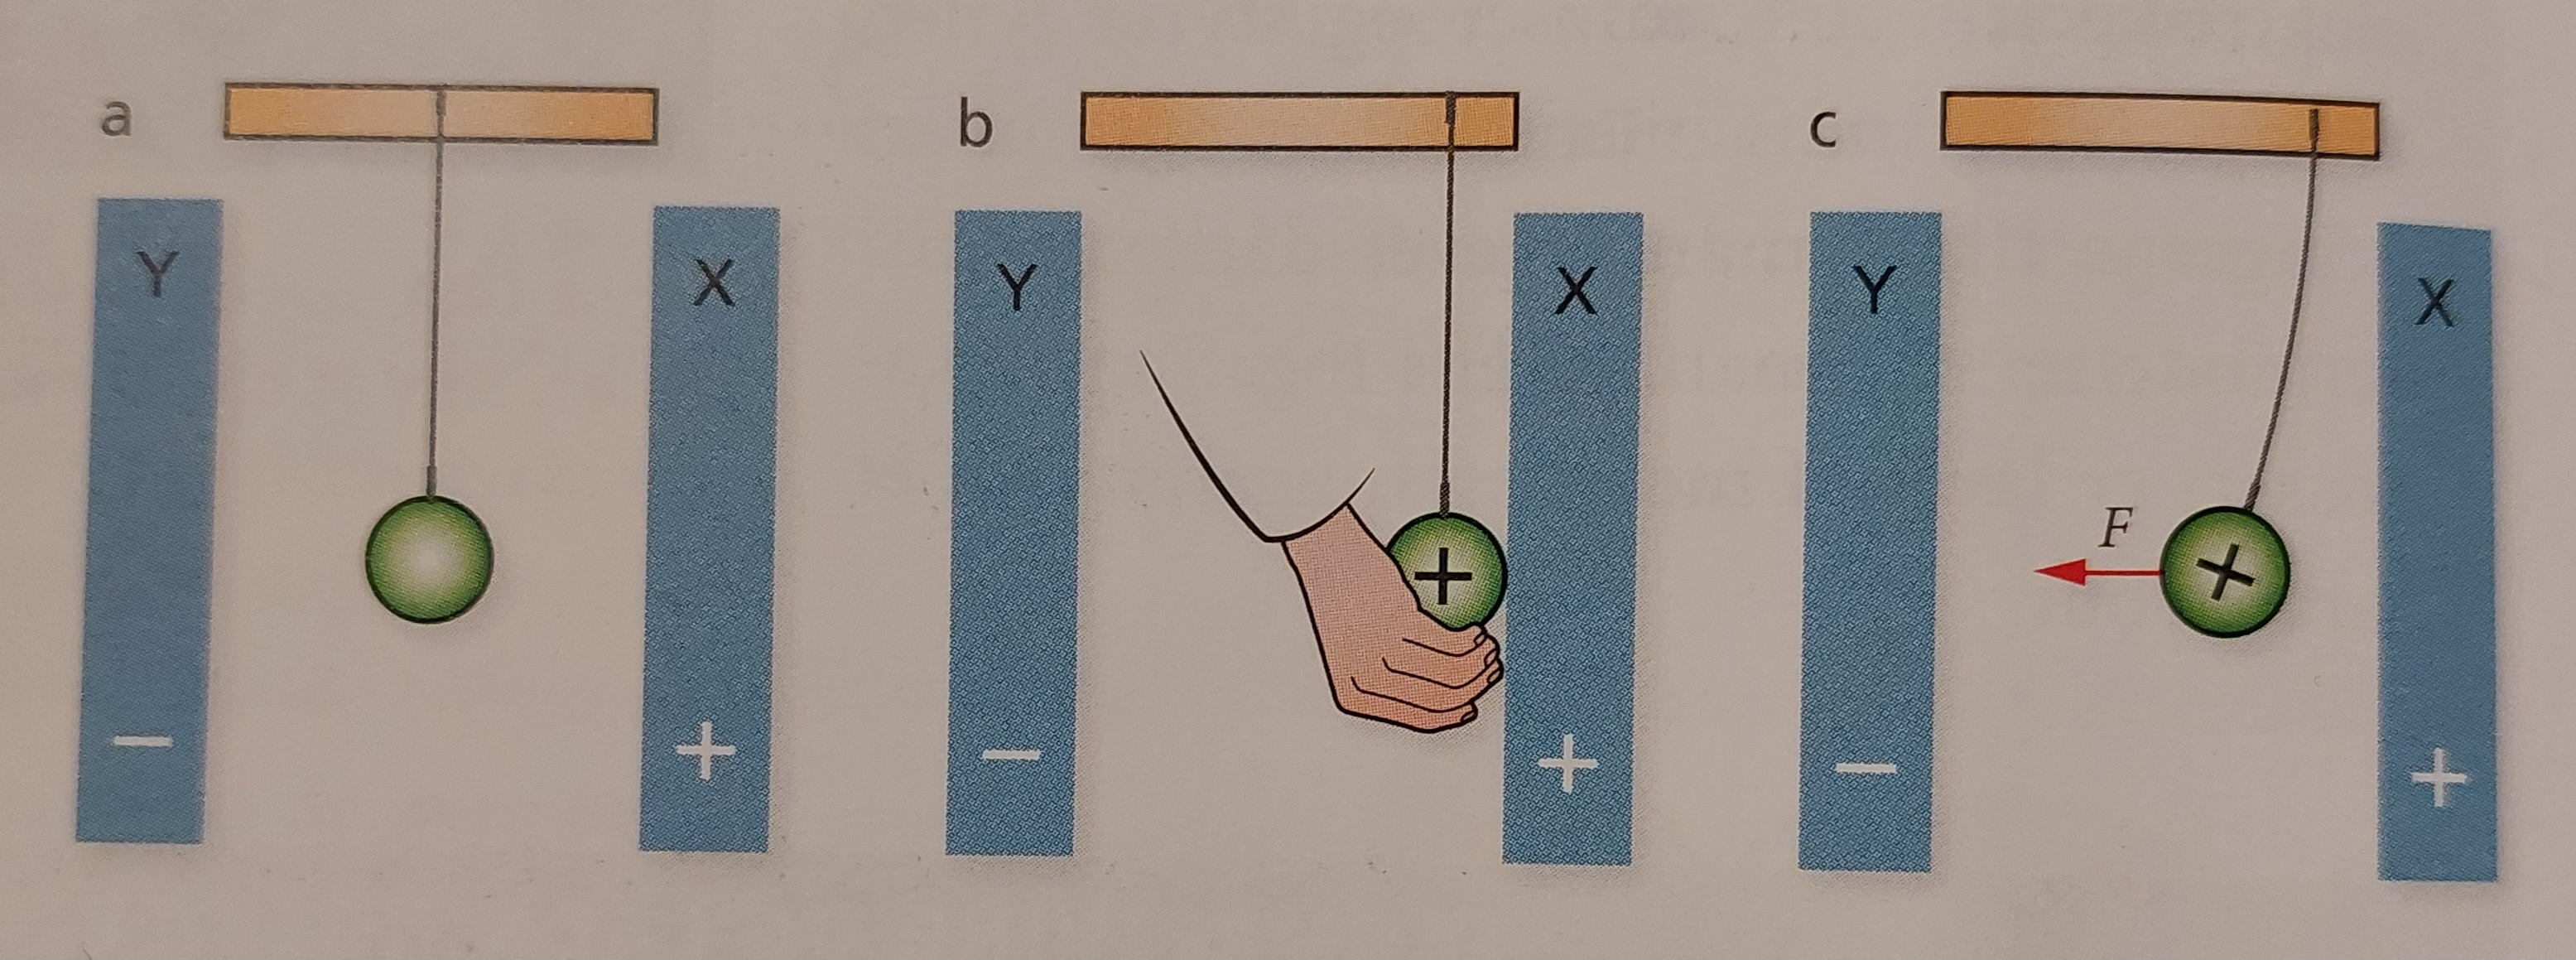
\includegraphics[width=.9\linewidth]{./img/spaendingsforskel.jpg}
\end{center}
\begin{itemize}
\item Neutral elektrisk ledende kugle lades op af den positive plade.
\item Den nu positivt elektrisk ladede kugle skubbes nu mod den negative plade.
\item Kuglen mister elektrisk \emph{potentiel} energi.
\item Tænk på gravitationel potentiel energi.
\end{itemize}
$$\boxed{U = \frac{\Delta E}{Q}}$$
\begin{itemize}
\item \(U\) kaldes \textbf{spændingen}, spændingsforskellen eller spændingsfaldet.
\item SI-enheden for spænding er volt \(\left[ U \right] = V\).
\end{itemize}

\subsubsection*{Opgaver}
\label{sec:org998825e}
\textbf{14.5}

En elektron, der gennemløber et spændingsfald på 1 V, får den elektriske energi \(E= 1 e \cdot 1 V\). Denne energi kaldes 1eV, kaldet \emph{elektronvolt}. \textbf{Omregn energi 1eV til joule.}

\textbf{14.7}

Bestem det spændingsfald, der skal til for at accelere en elektron op til 1 \% af lysets hastighed.
\textbf{14.6}

I et bestemt katodestrålerør gennemløber elektroner et spændingsfald på 10.0 kV.

\begin{enumerate}
\item Bestem den elektriske energi, en elektron tilføres, både i eV og J.
\item Hvad bliver elektronens hastighed, hvis den starter fra hvile? (Tip: Bestem først \(E_\text{kinetisk}\).
\end{enumerate}

\subsection*{Batterier}
\label{sec:org81be910}
\begin{center}
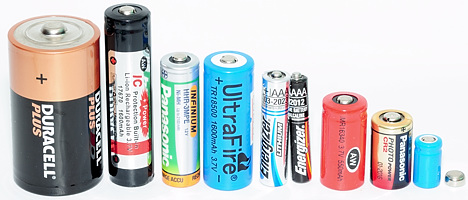
\includegraphics[width=.9\linewidth]{./img/batterier.jpg}
\end{center}

Eller
\href{https://youtu.be/\_yHJBDeshPA}{file:./img/master-of-puppets\_cover.webp}

\subsection*{Batterier}
\label{sec:orgc873675}
\begin{itemize}
\item Batteriet omdanner oplagret kemisk energi til elektrisk energi.
\item Batteriet "løfter" elektroner gennem batteriet og sørger for at erstatte polernes ladninger med nye ladninger.
\item Opbyg et elektrisk kredsløb bestående af et \textbf{batteri}, en elektriske \textbf{pære} og to \textbf{ledninger}.
\item Hvad kan man ændre på i netop denne opstilling?
\end{itemize}

\subsubsection*{Opgaver}
\label{sec:org8818421}
\textbf{14.8}

Et almindeligt bilbatteri kaldes en akkumulator. En akkumulators \emph{kapacitet} siger noget om, hvor stor en ladning der kan hentes ud af den, inden den behøver at oplades igen. Et bestemt 12 V-batteri har kapaciteten 44 Ah.

\begin{enumerate}
\item Hvor mange coulomb svarer 44 Ah til?
\item Hvor lag tid tager det at oplade batteriet, hvis strømstyrken er 2.0 A?
\item Ved normal brug er batteriets spænding nogenlunde konstant. Hvor stor elektrisk energi kan batteriet afgive, når det er fuldt opdaget?
\end{enumerate}
\textbf{14.9}

En gadelampe lyser ved hjælp af et batteri, der oplades af en solcelle. Lampen består af en serieforbindelse af LED-pærer og lyser ved en spænding på 12 V og strømstyrke på 8 A. Fuldt opladet kan batteriet indeholde ladningen 80 Ah.

\begin{enumerate}
\item Hvor mange timer kan lampen lyse, når batteriet er fuldt opladet?
\item Hvad er den samlede effekt af lampen?
\item Hvor stor elektrisk ladning passere batteriet, hvis lampen lyser i 5 timer?
\end{enumerate}

\subsection*{Energi og effekt}
\label{sec:orgaf3b3e6}
\begin{center}
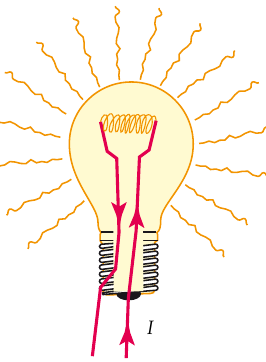
\includegraphics[width=.9\linewidth]{./img/energi_og_effekt.png}
\end{center}
\begin{itemize}
\item Elektroner i en ledning eller et kredsløb taber hele tiden energi, når de støder ind i metalionerne.
\item Denne energi omdannes til varme.
\item Der afsættes altså energi i ledningen/kredsløbet.
\end{itemize}
\begin{itemize}
\item Fra definition på spænding
$$U = \frac{\Delta E}{\Delta Q} \to \Delta E = U \cdot \Delta Q$$
\item Fra definitionen på strømstyrke
$$I = \frac{\Delta Q}{\Delta t} \to \Delta Q = I \cdot \Delta t$$
\item Sat sammen fås
$$\boxed{\Delta E = U \cdot I \cdot \Delta t \quad (\text{Joulse lov})}$$
\item Fra definitionen på effekt
$$P = \frac{\Delta E}{\Delta t}$$
\item fås
$$\boxed{P = U \cdot I}$$
\end{itemize}

\section*{Elektristiske kredsløb}
\label{sec:org8e7ac9d}
\end{document}
